\documentclass[conference,9pt,letterpaper]{IEEEtran}
\usepackage[T1]{fontenc}
\usepackage{newtxtext,newtxmath}
\usepackage{microtype}
\clubpenalty=10000
\widowpenalty=10000
\displaywidowpenalty=10000
\brokenpenalty=1000
\usepackage{graphicx}
\usepackage{booktabs}
\usepackage{amsmath}
\usepackage{array}
\usepackage{xcolor}
\usepackage{soul}
\DeclareRobustCommand{\pending}[1]{{\sethlcolor{yellow}\hl{#1}}}
\setlength{\abovecaptionskip}{3pt}
\setlength{\belowcaptionskip}{2pt}
\setlength{\intextsep}{6pt plus 1pt minus 1pt}
\setlength{\textfloatsep}{7pt plus 1pt minus 1pt}
\setlength{\floatsep}{6pt plus 1pt minus 1pt}
\usepackage{cite}
\usepackage{url}
\usepackage{stfloats}
\usepackage{balance}
\makeatletter
\patchcmd{\@BAlancecol}
 {\setbox\@leftcolumn=\vbox to \@tempdima}
 {\@tempdimb=\ht1\advance\@tempdimb by\dp1
  \ifdim\@tempdimb>\@tempdima\@tempdima=\@tempdimb\fi
  \@tempdimb=\ht3\advance\@tempdimb by\dp3
  \ifdim\@tempdimb>\@tempdima\@tempdima=\@tempdimb\fi
  \setbox\@leftcolumn=\vbox to \@tempdima}
 {\typeout{MECC: balance packing includes split-box depth.}}
 {\errmessage{Failed to patch balanced-column packing}}
% Stretch section and figure spacing instead of leaving unequal column tails.
\patchcmd{\@BAlancecol}{\unvbox1\vfil}{\unvbox1}
 {\typeout{MECC: balanced left column uses body glue.}}
 {\errmessage{Failed to patch left balance tail}}
\patchcmd{\@BAlancecol}{\vfil}{}
 {\typeout{MECC: balanced right column uses body glue.}}
 {\errmessage{Failed to patch right balance tail}}
\makeatother
\usepackage{capt-of}
\usepackage{float}
\usepackage{needspace}
\setcounter{dbltopnumber}{3}
\renewcommand{\dbltopfraction}{0.85}
\renewcommand{\textfraction}{0.10}
\newcommand{\mecc}{\textsc{MECC}}
\newcommand{\BH}{B_{\mathrm H}}
\newcommand{\BC}{B_{\mathrm C}}
\newcommand{\KH}{K_{\mathrm H}}
\newcommand{\KC}{K_{\mathrm C}}
\newtheorem{proposition}{Proposition}
\title{MECC: Single-GPU MoE Inference with\protect\\Compiler-Guided Three-Tier Expert Caching}
% Anonymous review copy: no author names or affiliation spacer rows.
\author{}
\usepackage[hidelinks]{hyperref}
\hypersetup{pdftitle={MECC: Single-GPU MoE Inference with Compiler-Guided Three-Tier Expert Caching},pdfauthor={}}
\begin{document}
\maketitle\flushbottom
\begin{abstract}
Expert offloading enables single-GPU inference for mixture-of-experts (MoE) models. Repeated HDD reads make expert residency a source of inference latency. We present MECC, the MoE Expert Cache Compiler, for profile-guided placement and joint HBM/CPU caching. Its compiler allocates slots by layer and emits the expert IDs used for initialization. The runtime promotes router-selected experts and retains displaced GPU weights in the host cache. The delivery path orders HDD reads and H2D copies before GPU consumption. On one A100, MECC gives 1.77$\times$ decode speedup over streaming on FP16 Mixtral-8x7B. The evaluated Mixtral perplexity is 3.427. The emitted residency plan connects initial expert placement to request-driven promotion and demotion. Joint retention reduces HDD demand by 73.9\% relative to independent caches.
\end{abstract}

\begin{IEEEkeywords}
Mixture of experts, single-GPU inference, expert offloading, three-tier caching, hardware/software co-design.
\end{IEEEkeywords}

\section{Introduction}
Mixture-of-experts (MoE) models scale parameter capacity through sparse expert activation~\cite{shazeer,switch,mixtral,deepseekmoe}. For example, Mixtral selects two of eight experts in each layer. A single-GPU deployment can use high-bandwidth memory (HBM), host memory, and a hard disk drive (HDD) to hold that pool. The selected expert's location determines its delivery path. HBM residents are ready for GPU execution; host residents require a host-to-device (H2D) copy; cold experts require an HDD read followed by H2D. Each selected expert executes once its weights are available in HBM. Prefill can reuse fetched weights across prompt rows, and decoding can reuse them across output tokens. On shared servers, a serving task manages its expert allocation alongside other jobs and model instances. We study how to distribute that allocation across layers and retain weights for recurring requests. All MoE layers share the HBM and host allowances. Increasing one layer's allocation leaves fewer slots for others. The value of another slot depends on the demand already covered in that layer. Placement therefore couples the layers' local request distributions to a shared storage allocation.



Expert parallelism places experts across GPUs~\cite{deepspeedmoe,tutel,flashmoedist}. Single-GPU systems combine expert paging and caching~\cite{offloading,swapmoe,moeinfinity,promoe} with CPU/GPU execution~\cite{fiddler,daop,lightning}. MoE-CORE combines layer-wise allocation, profile initialization, and online replacement with cross-layer prefetching~\cite{core}. It also supports substitution for eligible expert misses. SSD-LLaMA retains evicted expert weights in RAM and pipelines storage delivery alongside lossless compression and CPU/GPU work partitioning~\cite{ssdllama}. Edge FlashMoE studies cache replacement for storage-backed expert access~\cite{flashmoe}. Within such a hierarchy, initial placement and later admission affect different requests. A profile determines which weights are available when serving begins. GPU replacement then determines which weights remain on the host. Promoting a CPU expert frees a host slot for the expert evicted from HBM. Using that slot maintains the evicted expert's position in the reuse order. Figure~\ref{fig:intro} compares this joint rule with independent HBM/CPU caches on an A100. Joint retention gives 4.46$\times$ decode speedup over independent replacement and reduces HDD demand by 73.9\%. MECC also gives 1.77$\times$ speedup over streaming. These comparisons motivate retaining reusable expert weights across both memory tiers throughout serving.



\begin{figure}[!t]
\centering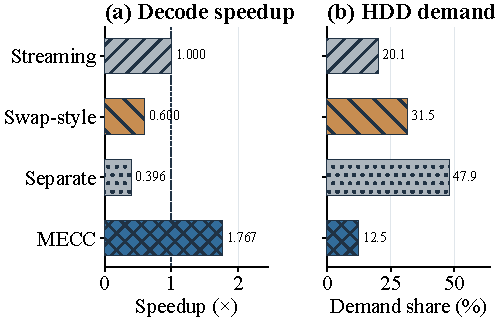
\includegraphics[width=\columnwidth]{measured_figures/intro_evidence.pdf}
\par\nointerlineskip
\caption{Mixtral-8x7B on one A100. Decode speedup is relative to streaming; Separate uses independent HBM/CPU caches. Swap-style is the SwapMoE-style adapter. Higher speedup and lower HDD demand are better.}
\label{fig:intro}
\end{figure}

We present \mecc{}, the MoE Expert Cache Compiler, to connect these two stages. Compilation ranks experts within each layer and allocates slots by marginal covered demand. The resulting plan specifies both per-layer capacities and the IDs loaded into HBM and CPU. The runtime maintains a joint recency order across those tiers. A CPU hit promotes the selected expert and demotes the GPU LRU expert; a cold admission can also evict a host resident. A host mirror supplies the weights of each demoted GPU resident. Host admission reuses this copy through a metadata update. Stream tracking keeps tensor storage live through kernel execution. Runtime requests update membership within the compiled capacities. Weight delivery follows the selected experts' read and copy dependencies before GPU execution. Prefill submits cold reads for the active expert batch, while decode loads selected experts on demand. The compiler and runtime address each weight block by its layer/expert ID. This key links profiled experts to placement, cache updates, and FP16~execution.

This paper makes three contributions.
\begin{list}{}{\setlength{\leftmargin}{16pt}\setlength{\labelwidth}{14pt}\setlength{\labelsep}{2pt}\setlength{\itemsep}{3pt}\setlength{\topsep}{3pt}}
\item[(1)] \textbf{Compiling initial residency.} We emit a model-specific residency plan containing per-layer capacities and ranked expert IDs. A marginal-coverage scan maps each additional slot to the demand it covers.
\item[(2)] \textbf{Updating cross-tier residency.} We connect the compiled state to promotion and GPU-to-host demotion. Host retention preserves GPU evictions for later reuse, while read/copy ordering prepares selected weights for consumption.
\item[(3)] \textbf{Evaluating weight delivery.} We compare placement, retention, and scheduling through decode latency, first-token time, source-tier demand, and sample perplexity. Workload and capacity sweeps examine calibration, task transfer, prompt length, batch size, and host allocation. Deployment comparisons report latency and accelerator occupancy.
\end{list}
\twocolumn[{
\begin{minipage}{\textwidth}
\centering
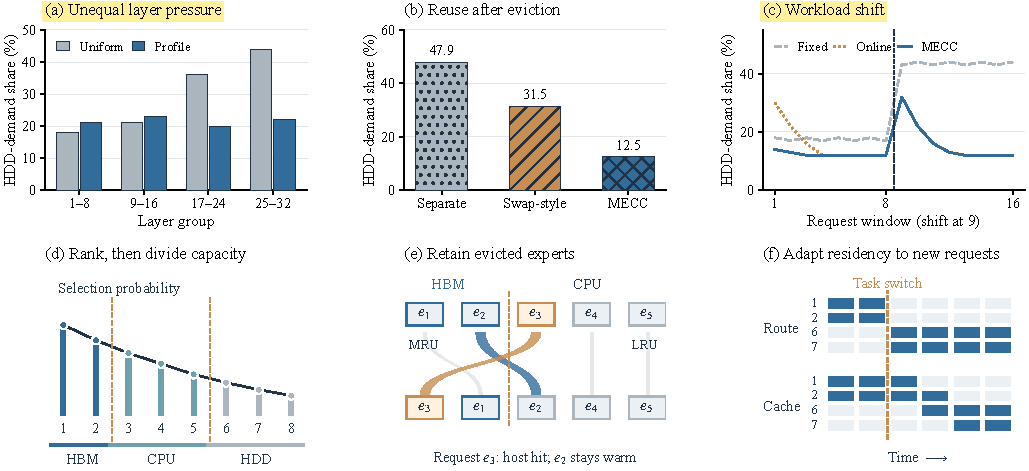
\includegraphics[width=\textwidth]{figures/fig02_motivation_insights.pdf}
\par\nointerlineskip
\captionof{figure}{Expert-cache behavior and MECC's three design choices. (a--c) compare layer pressure, cross-tier reuse, and workload change; (b) counts A100 demand across all phases. (d--f) show layer-specific capacity cuts, retention after GPU eviction, and online membership updates.}
\label{fig:insights}
\vspace{5pt}
\end{minipage}
}]
\balance
\section{Background}
\label{sec:background}
\subsection{Sparse Execution, Full Weight Capacity}
An MoE layer routes each token to a subset of experts and combines their outputs~\cite{shazeer,switch,gshard}. Mixtral and the DeepSeek family separate active computation from the size of the stored expert pool~\cite{mixtral,deepseekmoe,deepseekv2,deepseekv3,mixtral22}. An expert belongs to one layer; equal indices at different layers identify different weights. For input $x$, let $G(x)$ be the selected set and $g_e(x)$ its normalized gate weights. The layer computes
\begin{equation}
y(x)=\sum_{e\in G(x)}g_e(x)E_e(x).
\end{equation}
Each gate produces expert requests as a token traverses the model. Decode revisits the layers for each output token. An expert request triggers a residency lookup, weight delivery, and execution on its assigned token rows. The gate weights then combine the expert outputs.

\subsection{Expert Residency on One GPU}
Expert parallelism places experts on GPU owners and dispatches token activations to them~\cite{deepspeedmoe,tutel,megablocks,flashmoedist,harmoeny}. Single-GPU offloading delivers selected weights to the execution device. Experts share HBM with dense weights, activations, and the KV cache~\cite{pagedattention,sglang}. The host cache supplies H2D copies; HDD supplies weights absent from both resident tiers. Heterogeneous inference systems combine these paths with CPU/GPU scheduling~\cite{flexgen,dsinference,zeroinfinity,llmflash,powerinfer,hetegen}. In prefill, several prompt rows can share a fetched expert. Decode advances one token per sequence, exposing fewer rows to each active expert. The amount of ready computation therefore changes between the two phases. Other systems change transfer size through precision selection~\cite{hobbit,specter}, expert segmentation~\cite{moepic,slicemoe}, or staging and compression~\cite{mira,zipmoe}.

Calibration counts determine expert ranking; runtime accesses determine recency. Within one layer, sequences $[a,a,b,b]$ and $[b,b,a,a]$ have equal counts and different last-access orders. MECC initializes from the ranked profile and replaces residents by recency.

\section{Motivation and Insights}
\label{sec:challenges}
\subsection{Allocating Slots by Marginal Demand}
Expert demand varies across layers. Some layers concentrate requests in a few ranks; others spread requests across more experts. Figure~\ref{fig:insights}(a,d) illustrates the resulting allocation choice. Its profile-guided plan shifts slots toward the layer groups with more cold demand. The compiler makes this choice by comparing each layer's next uncovered rank. Allocating a slot exposes that layer's following rank as a new candidate. This process distributes a shared allowance across layers and retains the IDs that fill each allocation. Routing locality across models has also been studied independently~\cite{routingconsistency}.

\subsection{Preserving Reuse after GPU Eviction}
An expert evicted from the GPU can remain on the host. Figure~\ref{fig:insights}(b,e) shows a CPU promotion freeing a host slot for the GPU LRU expert. Joint retention fills that slot with the evicted expert and maintains its recency. Starting from the same allocation and expert order, joint retention reduces HDD demand from 47.9\% to 12.5\%. A demoted expert enters CPU MRU and remains available until subsequent admissions evict it from CPU LRU. A later selection promotes this host copy through H2D, turning the earlier GPU eviction into a host-cache hit.

\subsection{Updating Residency beyond Calibration}
Calibration and serving inputs can select different expert sets. In Figure~\ref{fig:insights}(c,f), a task switch moves requests toward a new expert set. MECC initializes the resident set from calibration and then admits experts requested during serving. Each admission updates recency and brings the cache closer to the active task. Repeated requests keep the new experts near MRU; their unused predecessors advance toward eviction. The profile supplies an initial hot set, and request-driven replacement tracks its evolution. The compiled capacities assign each layer the space used for this adaptation.

\twocolumn[{
\begin{minipage}{\textwidth}
\centering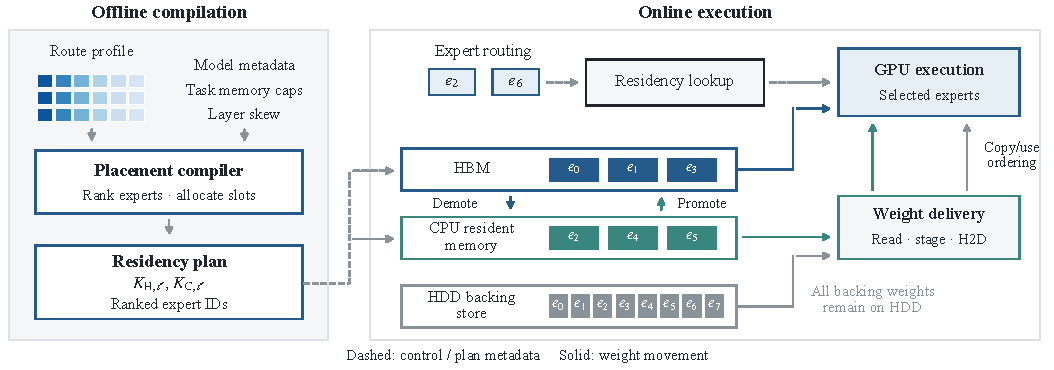
\includegraphics[width=\textwidth]{figures/fig01_overview.pdf}
\par\nointerlineskip
\captionof{figure}{MECC framework. The placement compiler emits per-layer capacities and ranked IDs. Online execution maps routed expert requests to HBM, CPU resident memory, or HDD, then supplies their weights to GPU computation. Dashed arrows carry control or plan metadata; solid arrows move weights.}
\label{fig:overview}

\vspace{8pt}
\end{minipage}
}]

\nobalance
\section{Overview}
\label{sec:overview}
Figure~\ref{fig:overview} follows the plan from profiling to GPU execution. The compiler receives layer/expert counts, skew parameters, model metadata, and expert allowances. It emits capacities and ranked IDs for each layer. Initialization loads the corresponding HBM and CPU residents; the complete expert pool remains on HDD. The runtime subsequently consumes this plan as an initial cache state.

Consider the selected experts $e_2$ and $e_6$ in the framework. The residency lookup finds $e_2$ on the host and $e_6$ in the backing store. Promoting $e_2$ frees a host slot for an expert evicted from HBM. Loading $e_6$ then admits another GPU resident and updates the same tier order. The delivery path resolves each weight's read and copy before its consumer executes. The model combines the expert outputs using the gate weights and continues to the next layer.

Residency persists across tokens. Each layer updates its own membership within the compiled capacities. Per-layer recency carries request history from one token to the next. Promotions refresh the active experts, and demotions extend their reuse through host residency. Section~\ref{sec:method} specifies these transitions; Section~\ref{sec:evaluation} examines the resulting delivery cost.

\section{Method}
\label{sec:method}
\subsection{Compiling Capacities and Initial Identities}
\begin{figure}[H]
\centering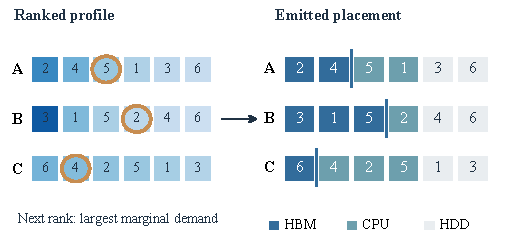
\includegraphics[width=\columnwidth]{method_redesign/compile_frontiers.pdf}
\par\nointerlineskip
\caption{Compiling the initial state. The left grid contains ranked per-layer demand; circles mark the next uncovered candidates. Shared HBM/CPU slot allowances produce different cuts in the emitted rows. A, B, and C identify different layers. }
\label{fig:compile}
\end{figure}

Consider $L$ MoE layers with $N_\ell$ experts per layer. For the routed pools considered here, experts have equal size $s$ and layers use the same top-$k$.

Expert allowances $B_{\mathrm H}$ and $B_{\mathrm C}$ provide $S_{\mathrm H}=\lfloor B_{\mathrm H}/s\rfloor$ HBM slots and $S_{\mathrm C}=\lfloor B_{\mathrm C}/s\rfloor$ CPU slots.

Calibration orders experts by selection counts. A log-count versus log-rank regression supplies $\alpha_\ell$ as the negative slope over positive counts. The rank model smooths this profile for allocation scoring:
\begin{equation}
q_{\ell,r}=\frac{r^{-\alpha_\ell}}{\sum_{j=1}^{N_\ell}j^{-\alpha_\ell}}.
\end{equation}
Here $q_{\ell,r}$ is conditional selection mass within layer $\ell$, with unit sum. Equal top-$k$ makes this mass comparable across layers. The expert IDs retain the count-derived order. E1 uses uniform allocation; E2 varies the profile and allocation inputs.

Figure~\ref{fig:compile} shows the HBM and CPU cuts in those lists. Capacities satisfy $\sum_\ell K_{\mathrm H,\ell}\le S_{\mathrm H}$, $\sum_\ell K_{\mathrm C,\ell}\le S_{\mathrm C}$, and $K_{\mathrm H,\ell}+K_{\mathrm C,\ell}\le N_\ell$. The adaptive scan reserves one slot per layer in each fast tier, then distributes the remaining slots by marginal coverage.

The scan first assigns HBM slots. At each step, it chooses the layer with the largest next-rank score:
\begin{equation}
\Delta_\ell=q_{\ell,K_{\mathrm H,\ell}+1}.
\end{equation}
CPU allocation continues from the first ranks beyond each HBM cut. Every allocation exposes a new next-rank candidate in that layer. Layer ID breaks score ties, and expert ID breaks count ties. The direct scan takes $O(L(S_{\mathrm H}+S_{\mathrm C}))$ time after sorting. Its score is the additional within-layer selection mass covered by the next slot.

The compiler serializes a residency plan: model dimensions, expert size, capacity arrays, and ranked layer-local IDs. Initialization loads each HBM prefix and the following CPU prefix. The JSON plan is the deployment artifact consumed by the loader. Admission subsequently updates membership within its capacities.

\subsection{Retaining Evicted Experts on the Host}
Each layer maintains two ordered sets, from most-recently used (MRU) to least-recently used (LRU). Their concatenation places HBM residents before CPU residents. An HBM hit moves its expert to HBM MRU. A CPU hit removes its host entry and promotes it to HBM MRU. The evicted GPU LRU expert then becomes CPU MRU. A cold admission follows the same GPU insertion and can remove the CPU LRU. HDD retains the backing weights for every expert.

\begin{figure}[H]
\centering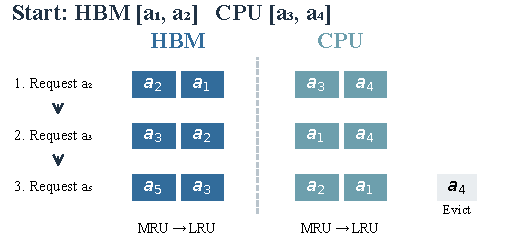
\includegraphics[width=\columnwidth]{method_redesign/residency_cases.pdf}
\par\nointerlineskip
\caption{A continuous request sequence, read from top to bottom. Each row starts from the preceding row's state. Request $a_2$ refreshes HBM recency; $a_3$ promotes from CPU; cold $a_5$ demotes $a_2$ and evicts $a_4$. All lists run MRU to LRU.}
\label{fig:retention}
\end{figure}
Figure~\ref{fig:retention} starts with HBM $[a_1,a_2]$ and CPU $[a_3,a_4]$. Request $a_2$ gives HBM $[a_2,a_1]$. Request $a_3$ then promotes $a_3$ and demotes $a_1$, producing HBM $[a_3,a_2]$ and CPU $[a_1,a_4]$. Finally, $a_5$ enters HBM, $a_2$ becomes CPU MRU, and $a_4$ leaves CPU LRU. The final lists are $[a_5,a_3]$ and $[a_2,a_1]$.

The resulting order extends from HBM MRU through CPU LRU. Requests enter at its front, and capacity pressure removes experts at its tail. During batch preparation, the loader can prepare several active experts. Temporary references hold their weights until each expert processes its token rows.

Each GPU resident carries a host mirror. Demotion admits this mirror to the CPU cache through a metadata update, saving a device-to-host copy. Tracking the consumer stream keeps tensor storage live until kernel execution completes.

\subsection{Ordering Delivery before Expert Consumption}
Prefill groups token rows by selected expert and submits the corresponding cold reads. Each read is resolved when its expert reaches consumption. Figure~\ref{fig:delivery} shows resident work overlapping a pending read for another selected expert. Decode delivers each requested expert on demand. The expert kernel processes its assigned rows, and the gate weights combine the resulting outputs.

\begin{figure}[H]
\centering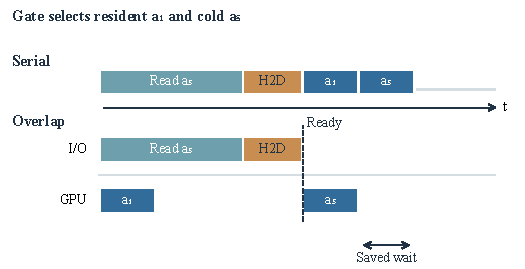
\includegraphics[width=\columnwidth]{method_redesign/delivery_overlap.pdf}
\par\nointerlineskip
\caption{Prefill delivery for resident $a_1$ and cold $a_5$. Computing $a_1$ overlaps the pending read for $a_5$. H2D completion releases $a_5$ for GPU execution; the shortened schedule saves exposed waiting time. }
\label{fig:delivery}
\end{figure}
A read future returns the host tensors that supply H2D. The copy stream moves them to the GPU and synchronizes before the loader yields the device tensors. The expert kernel then consumes those tensors. Recording its stream extends their lifetime through kernel completion. This read--copy--compute chain connects storage delivery to the expert's execution point.

Prefetchers use profiles or lookahead to anticipate expert demand~\cite{pregated,fate,expertflow}. Batch and request schedulers expose work from concurrent inputs~\cite{klotski,bevy}; distributed edge schemes add network delivery~\cite{odmoe}. MECC schedules the expert work already selected at the current gate. Retention removes repeated reads and copies. Overlap shortens the exposed part of the remaining delivery.

\section{Evaluation}
\label{sec:evaluation}
\subsection{Platform, Protocols, and Metrics}
The testbed has one A100 80~GB PCIe and a local HDD-backed RAID volume. FP16 Mixtral experts occupy 336~MiB each. Table~\ref{tab:protocols} defines the input and residency settings used throughout the evaluation. E1 uses uniform initialization; E2/E3 use calibrated initialization. E4 changes the host-slot allowance.

\begin{table}[H]
\centering
\caption{Execution protocols. Input/output are tokens per prompt. H/C are primary HBM/CPU allowances in GiB. E1/E4 use one run per point.}
\label{tab:protocols}
\setlength{\tabcolsep}{3pt}
\renewcommand{\arraystretch}{1.10}
\begin{tabular}{@{}lp{0.94in}p{0.70in}p{0.72in}@{}}
\toprule
ID & Input group & Prompts; tokens & H/C \\
\midrule
E1 & WikiText-2 & 8; 64/64 & 50/40 \\
\pending{E2} & GSM8K $\to$ HumanEval & 8+8; 128/128 & per model$^{a}$ \\
\pending{E3} & GSM8K, HumanEval & 8/task; 128/128 & per model$^{a}$ \\
E4 & WikiText-2 & 4; 64/16 & 50/30 or 60 \\
\pending{E5} & GSM8K, HumanEval & 8/task; 128/128 & 30/20 \\
\bottomrule
\end{tabular}
\par\smallskip
\raggedright $^{a}$Model-specific settings and figure-to-protocol mappings appear in Appendix~\ref{app:setup}.
\end{table}

TPOT measures decode time per output token; TTFT measures time to the first token. Phase speedup divides reference latency by policy latency, using full-precision run values. HDD-demand share is $n_D/(n_H+n_C+n_D+n_{\mathrm{CPUexec}})$. The main access counters aggregate warmup, prefill, decode, and PPL. Their denominator counts expert accesses, including batch-grouped accesses during prefill.

\subsection{Single-GPU Performance}
\begin{figure}[H]
\centering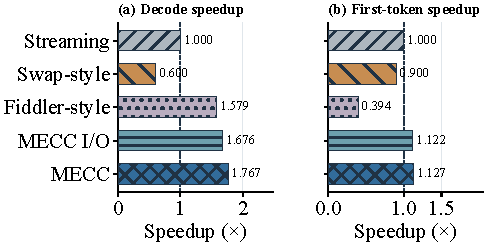
\includegraphics[width=\columnwidth]{measured_figures/main.pdf}
\par\nointerlineskip
\caption{Decode and first-token speedup on one A100, relative to streaming (1.0). Swap-style and Fiddler-style denote the corresponding mechanism adapters. MECC I/O varies the weight-delivery path. Higher is better.}
\label{fig:performance}
\end{figure}
E1 gives 1.77$\times$ decode and 1.13$\times$ first-token speedup over streaming in Figure~\ref{fig:performance}. Relative to Fiddler-style CPU computation, these ratios are 1.12$\times$ and 2.86$\times$. The phase-specific results distinguish first-token work from recurring expert delivery during generation.

E1 classifies 77.5\% of MECC accesses as HBM hits, 10.0\% as CPU hits, and 12.5\% as HDD accesses. Joint retention gives 2.95$\times$ decode speedup over the SwapMoE-style adapter and 4.46$\times$ over independent replacement. The independent-cache HDD share is 47.9\%. Figure~\ref{fig:intro} uses these aggregate counters.

On two short correctness inputs, MECC and streaming produce equal expert selections and greedy tokens. Maximum absolute logits and gate errors are zero across three output tokens per input. Appendix~\ref{app:setup} identifies the fixture and shared dispatch path.

\begin{figure*}[!t]
\centering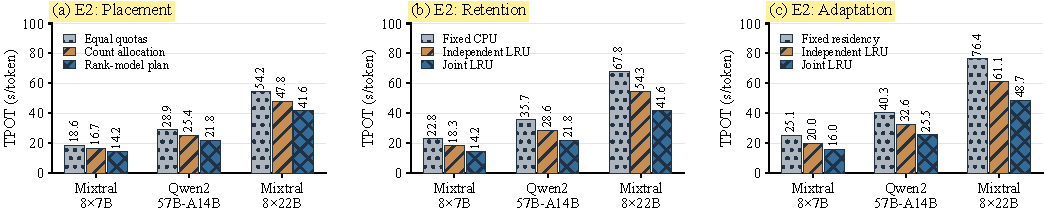
\includegraphics[width=\textwidth]{completion_figures/mechanism_sweeps.pdf}
\par\nointerlineskip
\caption{E2 allocation, retention, and adaptation across three models. Runtime policy is fixed in (a); initialization is fixed in (b,c). Bars report TPOT. }
\label{fig:target_mechanisms}
\end{figure*}
\Needspace*{12\baselineskip}
\balance
\subsection{Mechanism Attribution}
\label{sec:mechanisms}

E2 uses smaller resident allowances than E1 for Mixtral-8x7B. Figure~\ref{fig:target_mechanisms}(a) compares equal quotas, count allocation, and the rank-model plan. Their TPOT values are \pending{18.6, 16.7, and 14.2 s/token}. Panel (b) compares fixed CPU, independent LRU, and joint LRU at \pending{22.8, 18.3, and 14.2}. Panel (c) switches from eight GSM8K prompts to eight HumanEval prompts; joint admission changes post-switch TPOT from \pending{25.1 to 16.0}.

\begin{figure}[H]
\centering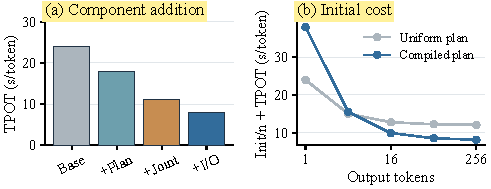
\includegraphics[width=\columnwidth]{completion_figures/ablation_startup.pdf}
\par\nointerlineskip
\caption{E3 ablation and initialization amortization. (a) Components under the GSM8K protocol. (b) Uniform versus compiled plans; curves sum amortized placement and decode time.}
\label{fig:target_ablation}
\end{figure}
For E3 Mixtral-8x7B/GSM8K, adding placement, joint retention, and delivery scheduling gives the TPOT sequence \pending{24, 18, 11, and 8 s/token} in Figure~\ref{fig:target_ablation}(a). The successive reductions are \pending{6, 7, and 3 s/token}. Joint retention provides the largest step by keeping evicted experts available on the host. Scheduling then shortens the delivery path at \pending{20 percent} HDD demand. Panel (b) includes the initial placement cost, connecting this decode gain to the response length.

\begin{figure}[H]
\centering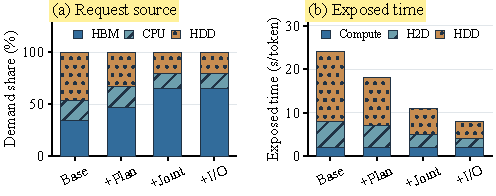
\includegraphics[width=\columnwidth]{completion_figures/traffic_exposure.pdf}
\par\nointerlineskip
\caption{E3 request sources and exposed delivery time. The final scheduling step changes exposed time at a fixed source distribution.}
\label{fig:target_traffic}
\end{figure}
Figure~\ref{fig:target_traffic} resolves the E3 component costs. HDD demand falls from \pending{46 to 20 percent}. The final scheduling step keeps the \pending{65/15/20 percent} HBM/CPU/HDD mix and changes TPOT from \pending{11 to 8 s/token}. Exposed HDD time falls by \pending{2 seconds} and H2D by \pending{1 second}. Retention removes transfers; scheduling shortens their exposed duration.

\subsection{Model and Deployment Scaling}
\begin{figure}[H]
\centering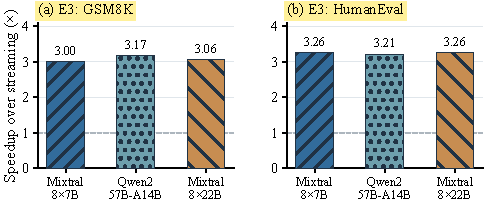
\includegraphics[width=\columnwidth]{completion_figures/cross_model.pdf}
\par\nointerlineskip
\caption{E3 model/workload comparison. GSM8K and HumanEval use 128 input and 128 output tokens, calibrated initialization, and the model-specific allowances in Table~\ref{tab:protocols}. }
\label{fig:target_models}
\end{figure}
Under E3 calibrated initialization, Figure~\ref{fig:target_models} gives streaming-to-MECC ratios of \pending{3.00--3.26}$\times$ across six model/workload groups. The absolute TPOT difference grows from \pending{16 seconds} on 8x7B/GSM8K to \pending{43 seconds} on 8x22B/HumanEval. Qwen2-57B-A14B gives \pending{3.17}$\times$ on GSM8K and \pending{3.21}$\times$ on HumanEval. E3 measures calibrated serving on these tasks. E1 evaluates uniform initialization on WikiText-2; its 1.77$\times$ ratio belongs to that configuration.

\begin{figure}[H]
\centering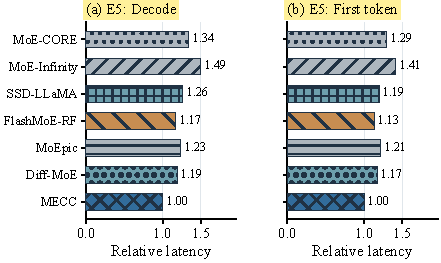
\includegraphics[width=\columnwidth]{completion_figures/matched_baselines.pdf}
\par\nointerlineskip
\caption{E5 candidate FP16 policy paths. Geometric means combine task-local latency ratios on GSM8K and HumanEval. MECC is 1.0; lower is better.}
\label{fig:matched}
\end{figure}
E5 compares profile-based placement, host retention, and history-based caching through the paths in Figure~\ref{fig:matched}. All paths use routed experts in FP16. Substitution and compression are disabled in this protocol. The comparison asks how the retention decision changes under a shared expert-store format and allowance. The candidates cover MoE-CORE, MoE-Infinity, SSD-LLaMA, FlashMoE-RF, MoEpic, and Diff-MoE~\cite{core,moeinfinity,ssdllama,flashmoe,moepic,diffmoe}. Appendix~\ref{app:setup} records each path and the full E1 adapter results.

\twocolumn[{
\begin{minipage}{\textwidth}
\centering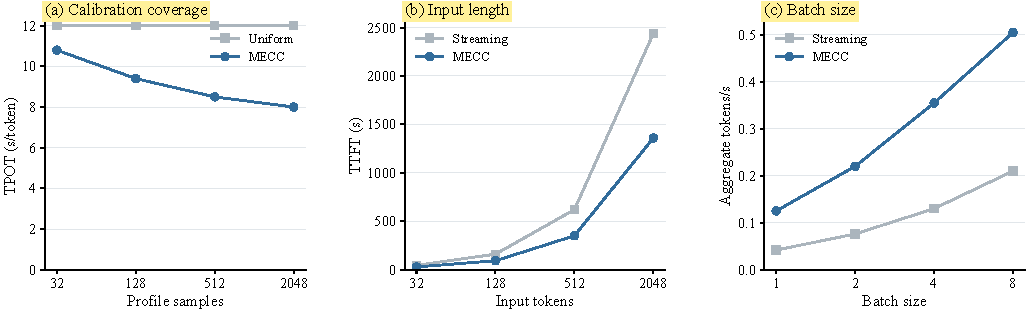
\includegraphics[width=\textwidth]{completion_figures/workload_sensitivity.pdf}
\par\nointerlineskip
\captionof{figure}{E7--E9 profile, input-length, and batch sensitivity. Profile size changes initialization quality, input length changes first-token work, and batch size changes aggregate throughput. The panels vary one workload parameter at a time.}
\label{fig:target_sensitivity}
\vspace{5pt}
\end{minipage}
}]
\balance
\subsection{Capacity and Workload Sensitivity}

E4 gives 1.42$\times$ and 5.17$\times$ speedup at 30 and 60~GiB CPU-slot allowances. Its four-prompt, 16-output-token protocol differs from E1. At 60~GiB, primary residency is 42~GiB in HBM plus 42~GiB on CPU: all 84~GiB of expert weights. Host mirrors add 42~GiB beyond the primary CPU pool. HDD demand falls from 32.2\% to zero. For a homogeneous pool, primary coverage is $L(K_H+K_C)s$. Physical host storage adds primary CPU weights, HBM mirrors, and staging. This accounts for the expert set and the copies that support demotion.

\begin{figure}[H]
\centering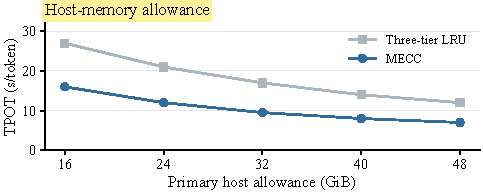
\includegraphics[width=\columnwidth]{completion_figures/quota_targets.pdf}
\par\nointerlineskip
\caption{E6 decode latency across primary host allowances; HBM allowance is 50 GiB.}
\label{fig:target_quota}
\end{figure}
Figure~\ref{fig:target_quota} sweeps primary host allowances from \pending{16 to 48 GiB}. MECC TPOT changes from \pending{16 to 7 s/token}, versus \pending{27 to 12} for three-tier LRU. Its first increment saves \pending{4 s/token}; the last saves \pending{1}. Earlier slots cover shorter reuse distances. E4 separately reaches complete expert coverage at 42~GiB HBM plus 42~GiB CPU residency.

\begin{figure}[H]
\centering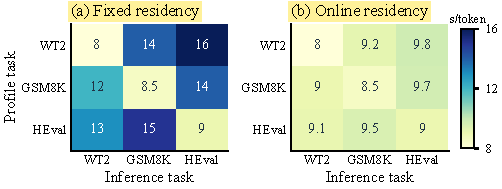
\includegraphics[width=\columnwidth]{completion_figures/profile_mismatch.pdf}
\par\nointerlineskip
\caption{E10 profile transfer across tasks. Rows select the calibration task and columns the inference task. Cells are TPOT in s/token; the two panels share a color scale.}
\label{fig:target_mismatch}
\end{figure}
Across Figure~\ref{fig:target_mismatch}'s six off-diagonal task pairs, fixed and online residency average \pending{14.00 and 9.38 s/token}, respectively. This gives a \pending{33.0 percent} reduction. Their diagonal means are both \pending{8.50 s/token}. Online admission adjusts the cached expert set to the serving task. Calibration size controls the initial profile.

\subsection{Calibration Coverage and Input Length}
Increasing calibration from \pending{32 to 2048 samples} changes TPOT from \pending{10.8 to 8.0 s/token} in Figure~\ref{fig:target_sensitivity}(a). The final expansion yields a smaller reduction than the first. Once the ranked hot set stabilizes, additional samples affect fewer initial placements.

Figure~\ref{fig:target_sensitivity}(b) varies input length from \pending{32 to 2048 tokens}. Endpoint first-token speedups are \pending{1.61}$\times$ and \pending{1.79}$\times$. At the longer input, TTFT is \pending{1360 seconds} for MECC and \pending{2440} for streaming. Prefill rows assigned to one expert share fetched weights and amortize delivery. Cache residency also reuses those weights across prompts.

\subsection{Batch Throughput and Sequence Progress}
Increasing batch size from \pending{one to eight} raises MECC's aggregate rate from \pending{0.125 to 0.505 tokens/s}, or \pending{4.04}$\times$, in Figure~\ref{fig:target_sensitivity}(c). For synchronous batches, the step interval is $B/R(B)$. These rates give \pending{8.00 and 15.84 seconds} at batches one and eight. The batch-step interval grows by \pending{1.98} times as the batch grows by \pending{8} times. Each step processes more rows and exposes more active expert work. Reporting both aggregate rate and step interval connects shared weight delivery to the progress of an individual sequence.

\subsection{Amortizing Initial Placement}
\label{sec:amortization}
Let $\Delta I$ be the extra initialization time and $\Delta D$ the per-token decode saving. The uniform/compiled plan control crosses at $n^\star=\Delta I/\Delta D$. Figure~\ref{fig:target_ablation}(b) uses \pending{18 seconds} of extra placement and \pending{4 seconds} of decode saving. The crossover is \pending{4.5 tokens}, so compiled placement pays off from the \pending{fifth token}.

At \pending{64 tokens}, placement-plus-decode averages are \pending{8.47 s/token} for the compiled plan and \pending{12.19} for uniform placement. For requests $j=1,\ldots,J$ sharing the cache, placement contributes $T_{\mathrm{init}}/\sum_j n_j$ per output token. Here $n_j$ is the output count of request $j$. Reusing the resident state pools these outputs into one amortization horizon. Reinitialization begins a new cache lifetime.

\section{Conclusion}
MECC compiles initial residency and carries expert reuse through joint HBM/CPU retention. The plan specifies capacities and expert IDs; runtime requests drive promotion, demotion, and delivery. State reuse amortizes initial placement across requests. E1 gives 1.77$\times$ decode speedup over streaming on one A100.

\clearpage
\balance
\bibliographystyle{IEEEtran}
\bibliography{references}
\clearpage
\appendices
\balance
\section{Experimental Configuration and Figure Data}
\label{app:setup}
\subsection{Platform and Physical Accounting}
The A100 exposes 80~GB HBM; the host has about 1~TB RAM. The backing volume is ext4 on RAID device /dev/sdb, reporting ROTA=1. Physical-drive inventory and isolated bandwidth were not recorded. HDD names this backing path throughout the draft.

Each expert occupies 352,321,536 bytes (336~MiB); the 256 experts total 84~GiB (90.19 decimal GB). Dense weights add to full-model size. E1 holds 128 HBM experts (42~GiB) and 96 CPU experts (31.5~GiB), plus 42~GiB of host mirrors. E4's 60~GiB CPU-slot allowance holds 128 CPU experts (42~GiB); mirrors bring host weights to 84~GiB before staging. Planner allowances constrain primary slots, not physical host usage. Legacy GB fields use GiB-sized slots.

\subsection{Protocol Map and Data Identity}
E1/E4 use committed single-A100 runs, one per policy/setting. E1 uses uniform initialization, eight WikiText-2 prompts at 64/64 tokens, and 1024-token PPL. E4 uses four prompts and 16 output tokens. Their 1.77$\times$ and 1.42$\times$/5.17$\times$ ratios describe distinct protocols.

Yellow values and panel titles identify authored, unmeasured design targets. E2/E3/E5 and secondary sweeps are not completed benchmark measurements. E2(a,b) use eight GSM8K prompts at 128/128 tokens; (c) adds eight HumanEval prompts after that window. Calibration uses 512 GSM8K samples. H/C allowances are 30/20~GiB for Mixtral-8x7B, 30/16 for Qwen2-57B-A14B, and 50/64 for Mixtral-8x22B. Allocation controls use equal quotas, empirical counts, or Zipf-smoothed ranks under the same runtime. Retention/adaptation share initial membership and capacities.

E3 uses the same token lengths, eight prompts per task, and 2048 calibration samples. H/C allowances are 50/40, 30/16, and 50/64~GiB for those three models. Its 3.00--3.26$\times$ ratios differ from E1's configuration. E3's scheduling step is a target extension; current decode delivers experts on demand.

E5 uses Mixtral-8x7B at 30/20~GiB, eight 128/128-token prompts per task, and 512 calibration samples. Task-local phase ratios on GSM8K/HumanEval are combined geometrically. All six baseline entries are authored targets for candidate local adaptations, not executions of the authors' systems or observed wins. They do not replace the E1 RF observation. MoEpic's entry is a whole-expert allocation control, excluding its split-expert system. Diff-MoE still requires full-text and implementation checks. Substitution, quantization, and compression are excluded. EXPERIMENT\_TARGETS.json stores task ratios and new Qwen2 points; original arrays remain archived.

E6--E10 inherit E3 8x7B/GSM8K defaults: 50/40~GiB, eight 128/128-token prompts, 2048 profile samples, and batch one. They vary host allowance, profile size, input length, batch, and calibration/serving task, respectively. E10 covers WikiText-2/GSM8K/HumanEval. All target configurations require implementation and hardware checks.

\subsection{Complete E1 Results and Controls}
E1 TPOT in seconds is 13.04259 (streaming), 21.75165 (SwapMoE-style), 8.25899 (Fiddler-style), 7.19497 (FlashMoE-RF), 7.78096 (MECC I/O), 7.38198 (MECC), and 32.94189 (independent). Streaming/MECC TTFT is 156.85501/139.14026 seconds; Fiddler-style TTFT is 398.446. Unrounded ratios give 4.46247$\times$ independent/MECC decode and 2.86363$\times$ Fiddler/MECC TTFT. FlashMoE-RF gives 1.81$\times$/1.54$\times$ decode/first-token speedup over streaming; MECC gives 1.77$\times$/1.13$\times$.

Streaming retains initialized GPU residents. SwapMoE-style fixes CPU residents and uses GPU LRU. Fiddler-style executes non-HBM experts on CPU. RF uses equal-weight inverse-recency/frequency scoring and GPU LRU, without the original trained predictor. These are local mechanism adapters. GPU PPL is 3.427; CPU-compute PPL is 3.432. Each point has one run and no variance estimate. Original run hashes remain in RATIO\_AUDIT.json.

\subsection{Counters, Calibration, and Correctness}
Main HDD shares aggregate expert accesses across warmup, prefill, decode, and PPL. MECC counts are 29,558 HBM, 3,820 CPU, and 4,764 HDD: 38,142 total. Prefetch is classified at consumption; initialization is excluded. Physical read/H2D bytes use separate counters. Target stacks sum to 100\%.

The allocator consumes skew parameters and count-ranked IDs. Profiling regresses positive log-counts on log-ranks; Mixtral fit residuals are unavailable. E1 uses uniform initialization; the non-uniform CLI generates skew unless explicit compiler input supplies it. The plan is serialized configuration, not GPU kernel code.

G1 compares streaming/MECC through shared dispatch on two 21/22-token inputs, three greedy outputs each, and 128-token PPL. Route/token equality is true; gate/logits maximum errors are 0.0. This is short-window path equality, not independent full-resident equivalence. GSM8K/HumanEval task accuracy remains unmeasured. G1\_EVIDENCE.json identifies the source Git object and hashes.

\subsection{Arithmetic and Deployment Scenario}
Fixed off-diagonal transfer cells sum to 84 (mean 14.00); online cells sum to 56.3 (mean 9.3833), a 32.976\% reduction. Uniform/compiled startup uses 12/30-second placement and 12/8-second decode, crossing at 4.5 tokens. Curves exclude prefill. Compiled decode matches E3 GSM8K, E6 at 40~GiB, E7 at 2048 samples, and E9 at batch one. Figure~\ref{fig:target_gpu} contains authored deployment targets.

\begin{figure}[H]
\centering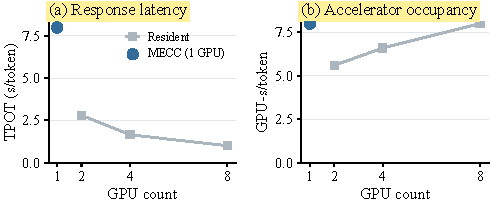
\includegraphics[width=\columnwidth]{completion_figures/gpu_tradeoff.pdf}
\par\nointerlineskip
\caption{Deployment scenario: latency and accelerator occupancy for one-GPU MECC and resident references. Yellow titles follow the target-array convention above.}
\label{fig:target_gpu}
\end{figure}
\end{document}
